\documentclass{article}

\usepackage{arxiv}

\usepackage[utf8]{inputenc}
\usepackage[T1]{fontenc}
\usepackage{natbib}
\usepackage[french]{babel}
\usepackage{hyperref}
\usepackage{url}
\usepackage{booktabs}
\usepackage{multirow}
\usepackage{amsfonts}
\usepackage{amsmath}
\usepackage{nicefrac}
\usepackage{microtype}
\usepackage{graphicx}
\usepackage{subcaption}
\usepackage{float}
\setlength{\textfloatsep}{6pt plus 2pt minus 2pt}
\setlength{\floatsep}{6pt plus 2pt minus 2pt}
\setlength{\intextsep}{6pt plus 2pt minus 2pt}
\setlength{\abovecaptionskip}{4pt}
\setlength{\belowcaptionskip}{2pt}
\raggedbottom
\usepackage{doi}

\title{Analyse Préliminaire --- Apprentissage par renforcement sur \textit{FrozenLake}}

\newif\ifuniqueAffiliation
\uniqueAffiliationtrue

\ifuniqueAffiliation
\author{
  Ibrahim R. HADJ-ARAB \\
  Faculté des sciences et de génie\\
  Université Laval\\
  \texttt{ibrahim-rabah.hadj-arab.1@ulaval.ca} \\
  \And
  Khalil EN NOUAARY \\
  Faculté des sciences et de génie\\
  Université Laval\\
  \texttt{khalil.en-nouaary.1@ulaval.ca} \\
}
\fi

\renewcommand{\shorttitle}{Analyse Préliminaire --- IFT-7201}

\hypersetup{
  pdftitle={Analyse préliminaire RL sur FrozenLake},
  pdfauthor={Ibrahim R. Hadj-Arab, Khalil En Nouaary},
}

\begin{document}
\maketitle

\noindent Code source disponible à : \url{https://github.com/Ribraba/IFT-7201-Projet}

\section{Cas d'étude}

\subsection{Composantes de l'environnement}

\textit{FrozenLake-v1}~\citep{towers2024} est un environnement de navigation en grille $N \times N$. L'espace d'états est l'ensemble des $N^2$ cases ; l'espace d'actions contient quatre déplacements (haut, bas, gauche, droite). Trois composantes peuvent être manipulées pour moduler la difficulté de l'environnement et l'exposition aux situations dangereuses :

\begin{itemize}
  \item \textbf{Degré de stochasticité.} Le paramètre \texttt{is\_slippery} contrôle la dynamique de transition. Lorsque activé, chaque action entraîne le déplacement souhaité avec probabilité $\nicefrac{1}{3}$ et l'un des deux déplacements perpendiculaires avec probabilité $\nicefrac{1}{3}$ chacun, rendant l'environnement non-déterministe.
  \item \textbf{Nombre de situations dangereuses.} Les cases de type \texttt{H} (trous) constituent les situations dangereuses. Augmenter leur nombre réduit la surface praticable et multiplie les risques de chute.
  \item \textbf{Positionnement des situations dangereuses.} Regrouper les trous de façon contiguë (ex.\ rangée horizontale) crée un obstacle de type falaise, forçant l'agent à choisir entre un chemin court risqué et un détour sûr.
\end{itemize}

La fonction de récompense est mise en forme pour accélérer la propagation du signal de danger : chute dans un trou ($r = -1{,}0$), atteinte de l'objectif ($r = +1{,}0$), collision avec un mur ($r = -0{,}1$), déplacement ordinaire ($r = 0{,}0$).

\subsection{Cas d'étude}

\begin{figure}[h]
  \centering
  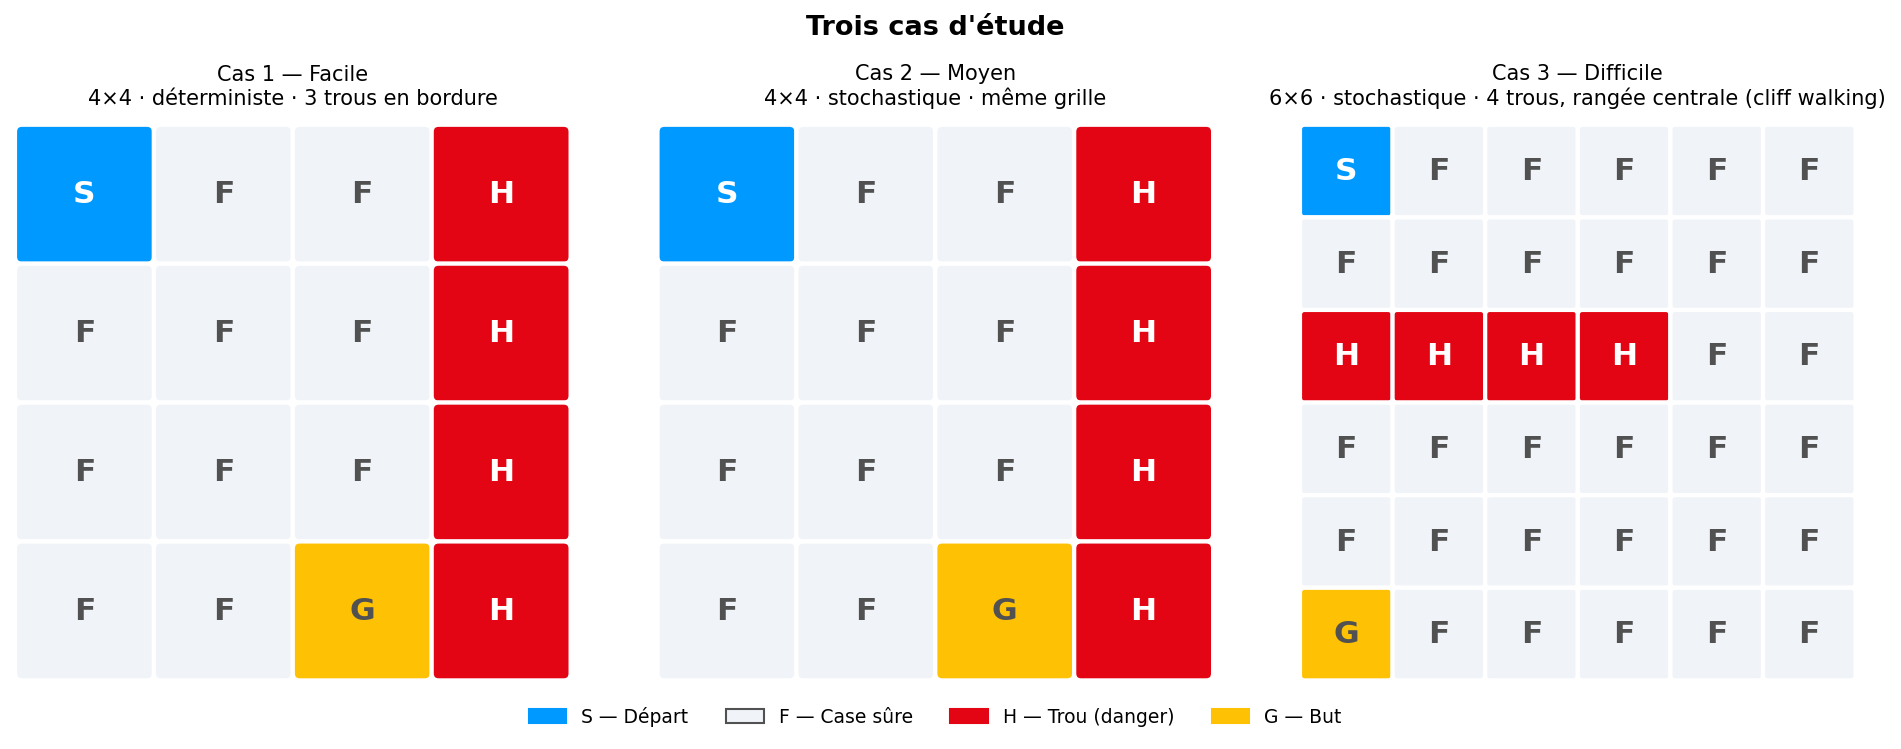
\includegraphics[width=\linewidth]{../figures/maps.png}
  \caption{Visualisation des trois environnements. \texttt{S}~: départ, \texttt{G}~: objectif, \texttt{H}~: trou (situation dangereuse), \texttt{F}~: case libre.}
  \label{fig:maps}
\end{figure}

Le Tableau~\ref{tab:configs} et la Figure~\ref{fig:maps} présentent les trois configurations retenues.

\begin{table}[h]
  \centering
  \caption{Configurations des trois cas d'étude.}
  \label{tab:configs}
  \small
  \begin{tabular}{lccc}
    \toprule
    & \textbf{Facile} & \textbf{Moyen} & \textbf{Difficile} \\
    \midrule
    Taille de la grille          & $4\times4$ & $4\times4$ & $6\times6$ \\
    \texttt{is\_slippery}        & Non & Oui & Oui \\
    Nombre de trous              & 3   & 3   & 4 \\
    Positionnement               & Colonne droite & Colonne droite & Rangée centrale \\
    Position de l'objectif       & Bas-centre & Bas-centre & Bas-gauche \\
    \bottomrule
  \end{tabular}
\end{table}

\textbf{Facile} ($4\times4$, déterministe, 3 trous en colonne). Les transitions sont déterministes. Ce cas sert de référence : en l'absence de bruit, toute stratégie TD doit converger vers un taux de chutes nul et un taux de boucles nul. Il valide l'implémentation et établit une borne supérieure de performance.

\textbf{Moyen} ($4\times4$, stochastique, 3 trous en colonne). Topologie identique à \textit{Facile} ; seul \texttt{is\_slippery} change. Ce cas isole rigoureusement l'effet de la stochasticité : toute dégradation de performance est attribuable uniquement au non-déterminisme, non à la topologie de la grille.

\textbf{Difficile} ($6\times6$, stochastique, 4 trous contigus en rangée centrale, objectif en bas-gauche). La rangée \texttt{HHHHFF} crée une barrière horizontale analogue au problème du \textit{cliff walking}~\citep[chap.~6]{sutton2018}. L'objectif étant placé en bas-gauche, directement au-dessous de la barrière, deux trajectoires coexistent : un chemin court risqué descendant par la colonne gauche (en bordure des trous) et un long détour sûr contournant la barrière par les colonnes droites. Le passage à la grille $6\times6$ est délibéré : il augmente l'espace d'états pour que le détour sûr soit significativement plus long que le chemin risqué, condition nécessaire pour que la divergence \textit{off-policy}/\textit{on-policy} soit observable et mesurable par l'algorithme de Dijkstra.


\section{Stratégies considérées}

Deux stratégies de différence temporelle (TD) sont sélectionnées comme baselines : Q-learning et SARSA. Ces méthodes ne disposent d'aucun mécanisme conçu explicitement pour éviter les situations dangereuses, ce qui permet d'établir une limite de référence que toute stratégie de sécurité ultérieure devra dépasser. Le choix de méthodes tabulaires (plutôt que DQN~\citep{mnih2015} ou PPO) est justifié par la taille réduite de l'espace d'états ($4\times4 = 16$ et $6\times6 = 36$ états) : les méthodes tabulaires convergent vers la solution exacte sans approximation de fonction, ce qui garantit que les différences observées reflètent bien les propriétés intrinsèques des algorithmes. De plus, Q-learning et SARSA forment la paire canonique \textit{off-policy} / \textit{on-policy} dont les comportements divergents face aux obstacles sont directement prédits par la théorie~\citep{sutton2018}.

\textbf{Q-learning}~\citep{watkins1992} est une méthode \textit{off-policy} dont la règle de mise à jour repose sur la valeur maximale de l'état suivant :
\begin{equation}
  Q(s, a) \leftarrow Q(s, a) + \alpha \bigl[r + \gamma \max_{a'} Q(s', a') - Q(s, a)\bigr].
\end{equation}
Cette mise à jour optimiste suppose que la politique optimale sera suivie dans le futur, indépendamment de l'exploration en cours. Dans des environnements à obstacles groupés, cette hypothèse peut conduire à sous-estimer le risque réel de chute et à préférer le chemin court risqué.

\textbf{SARSA}~\citep{rummery1994} est une méthode \textit{on-policy} qui utilise l'action réellement sélectionnée selon la politique $\varepsilon$-greedy courante :
\begin{equation}
  Q(s, a) \leftarrow Q(s, a) + \alpha \bigl[r + \gamma\, Q(s', a') - Q(s, a)\bigr].
\end{equation}
Puisque $a'$ peut être une action aléatoire (avec probabilité $\varepsilon$), SARSA intègre le coût de l'exploration dans ses estimations. On s'attend donc à ce qu'il apprenne à éviter davantage les cases proches des trous, au prix d'une propagation plus lente du signal de danger en début d'apprentissage. La confrontation de ces deux comportements opposés face au risque est la principale motivation de leur sélection.


\section{Méthodologie expérimentale}

\textbf{Librairies.} L'environnement est fourni par Gymnasium~1.2.3~\citep{towers2024}. Q-learning et SARSA sont implémentés directement en Python/NumPy~2.2.6, sans recours à Stable-Baselines3~\citep{raffin2021}, afin de contrôler précisément les mises à jour TD.

\textbf{Hyper-paramètres.} Les deux algorithmes partagent : $\gamma = 0{,}99$ (horizon long, adapté aux trajectoires multi-étapes jusqu'à l'objectif), $\alpha_0 = 0{,}5$ (valeur standard pour les méthodes TD tabulaires~\citep{sutton2018}), décroissance $0{,}9995$ pour $\alpha$ et $\varepsilon$ jusqu'aux minima $\alpha_{\min}=0{,}01$ et $\varepsilon_{\min}=0{,}05$. Ce taux de décroissance amène $\varepsilon$ à son minimum après $\approx\!6\,000$ épisodes, assurant une phase d'exploration large suivie d'une exploitation progressive sur les 14\,000 épisodes restants.

\textbf{Paramètres expérimentaux.} Chaque configuration est entraînée sur 20\,000 épisodes, avec un maximum de 200 pas par épisode. Les expériences sont répétées avec $n=10$ graines indépendantes (graines 0 à 9) pour produire des intervalles de confiance (moyenne $\pm$ écart-type). L'évaluation finale utilise la politique greedy ($\varepsilon=0$) sur 500 épisodes.

\textbf{Indicateurs de performance.} L'étude évalue la sécurité \emph{durant} l'apprentissage et sur la politique finale. Cinq indicateurs sont mesurés :
\begin{itemize}
  \item \textbf{Récompense cumulée durant l'entraînement} : indicateur de convergence de la politique (moyenne mobile, fenêtre 500 épisodes).
  \item \textbf{Taux de chutes durant l'entraînement} : fraction d'épisodes terminés dans un trou. Mesure la sécurité au cours de l'apprentissage.
  \item \textbf{Taux de boucles durant l'entraînement} : fraction d'épisodes terminés par dépassement du nombre maximal de pas. Distingue l'échec par danger (chute) de l'échec par inefficacité (blocage) — un agent qui évite les trous mais reste circulaire n'est pas opérationnel.
  \item \textbf{Taux d'états dangereux à l'évaluation} : fraction de pas passés dans une case adjacente à un trou lors de l'évaluation greedy ($\varepsilon=0$). Quantifie la proximité aux obstacles de la politique finale.
  \item \textbf{Taux de chemins sécurisés à l'évaluation} : fraction des épisodes réussis dont la trajectoire chevauche à au moins 50\,\% le chemin optimal de sécurité, calculé par une variante de Dijkstra~\citep{dijkstra1959} pénalisant les cases adjacentes à un trou (cas Difficile uniquement). Quantifie la capacité de la politique finale à emprunter le détour sûr.
\end{itemize}

\section{Résultats}
\begin{figure}[H]
  \centering
  \begin{subfigure}[t]{0.47\linewidth}
    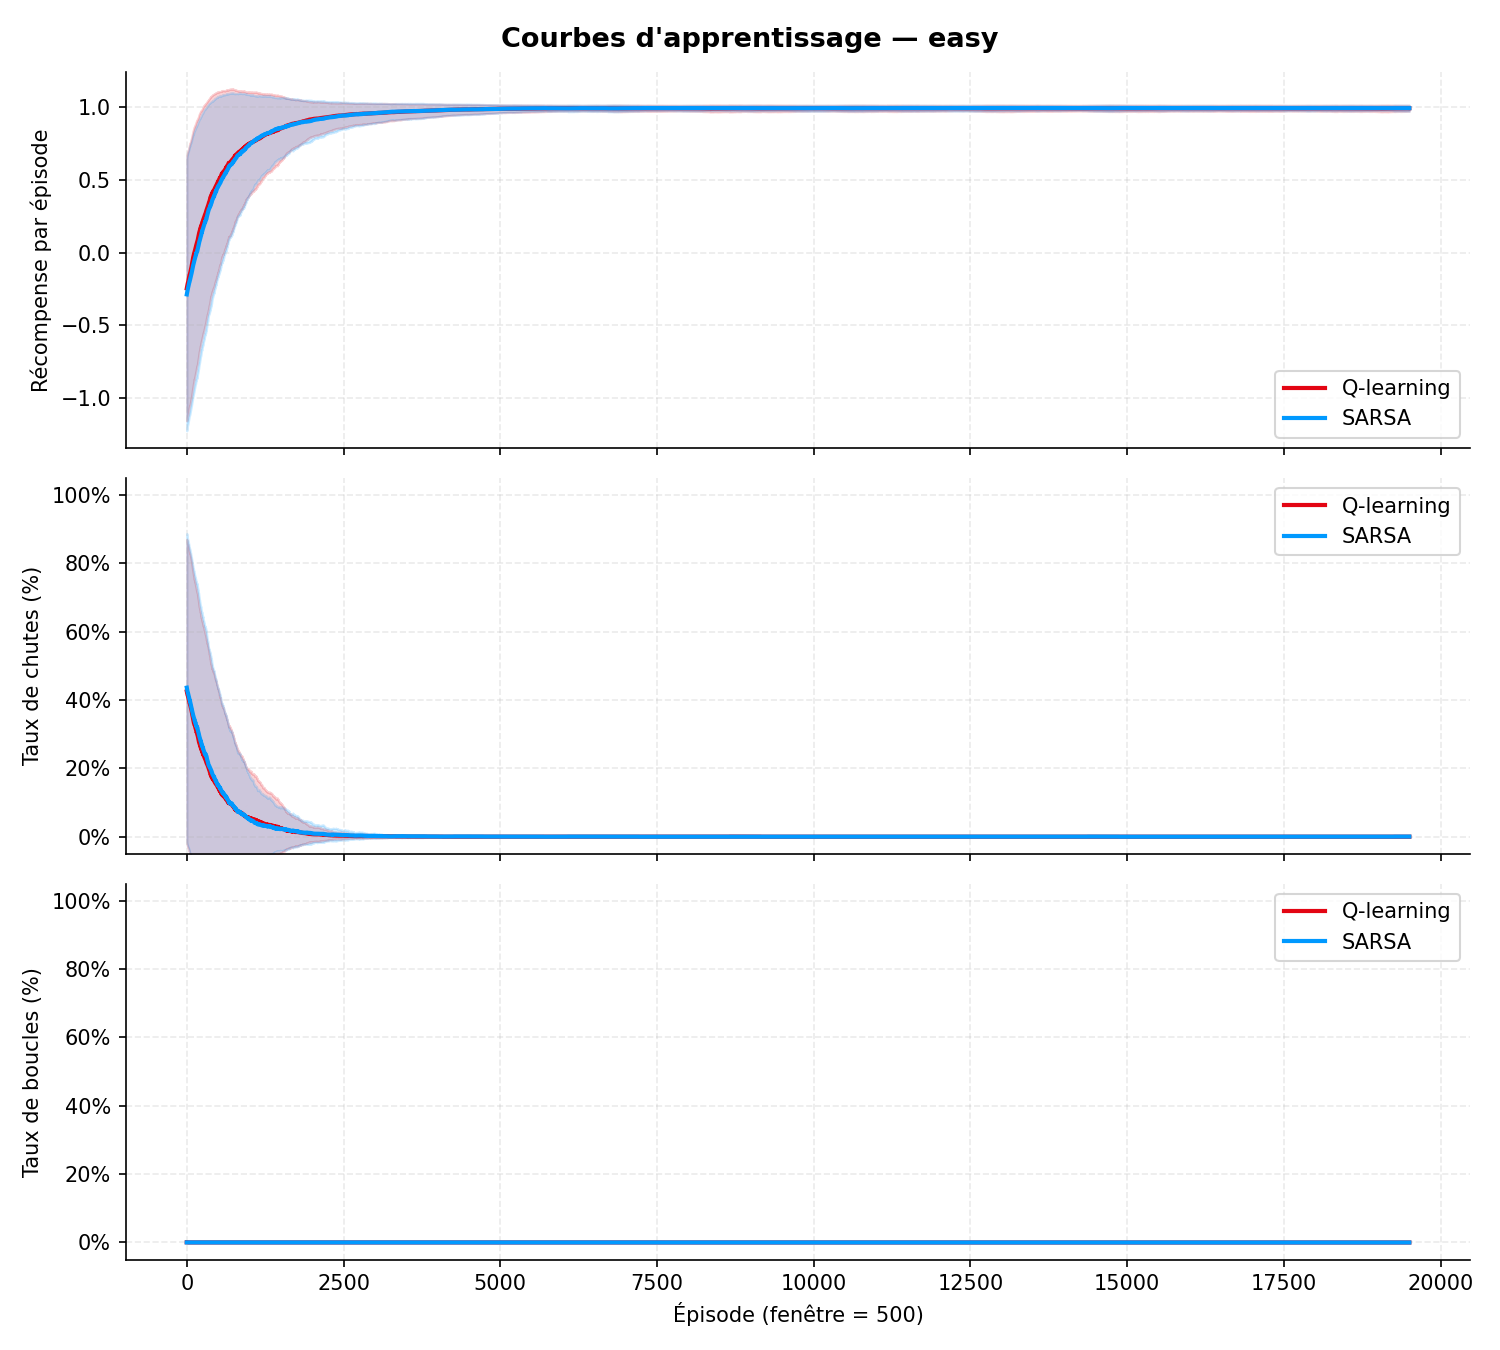
\includegraphics[width=\linewidth]{../figures/training_easy.png}
    \caption{\textbf{Facile} --- Convergence vers 0\,\% de chutes et 0\,\% de boucles dès $\approx\!2\,000$ épisodes. Valide les deux implémentations en environnement déterministe.}
    \label{fig:train_easy}
  \end{subfigure}
  \hfill
  \begin{subfigure}[t]{0.47\linewidth}
    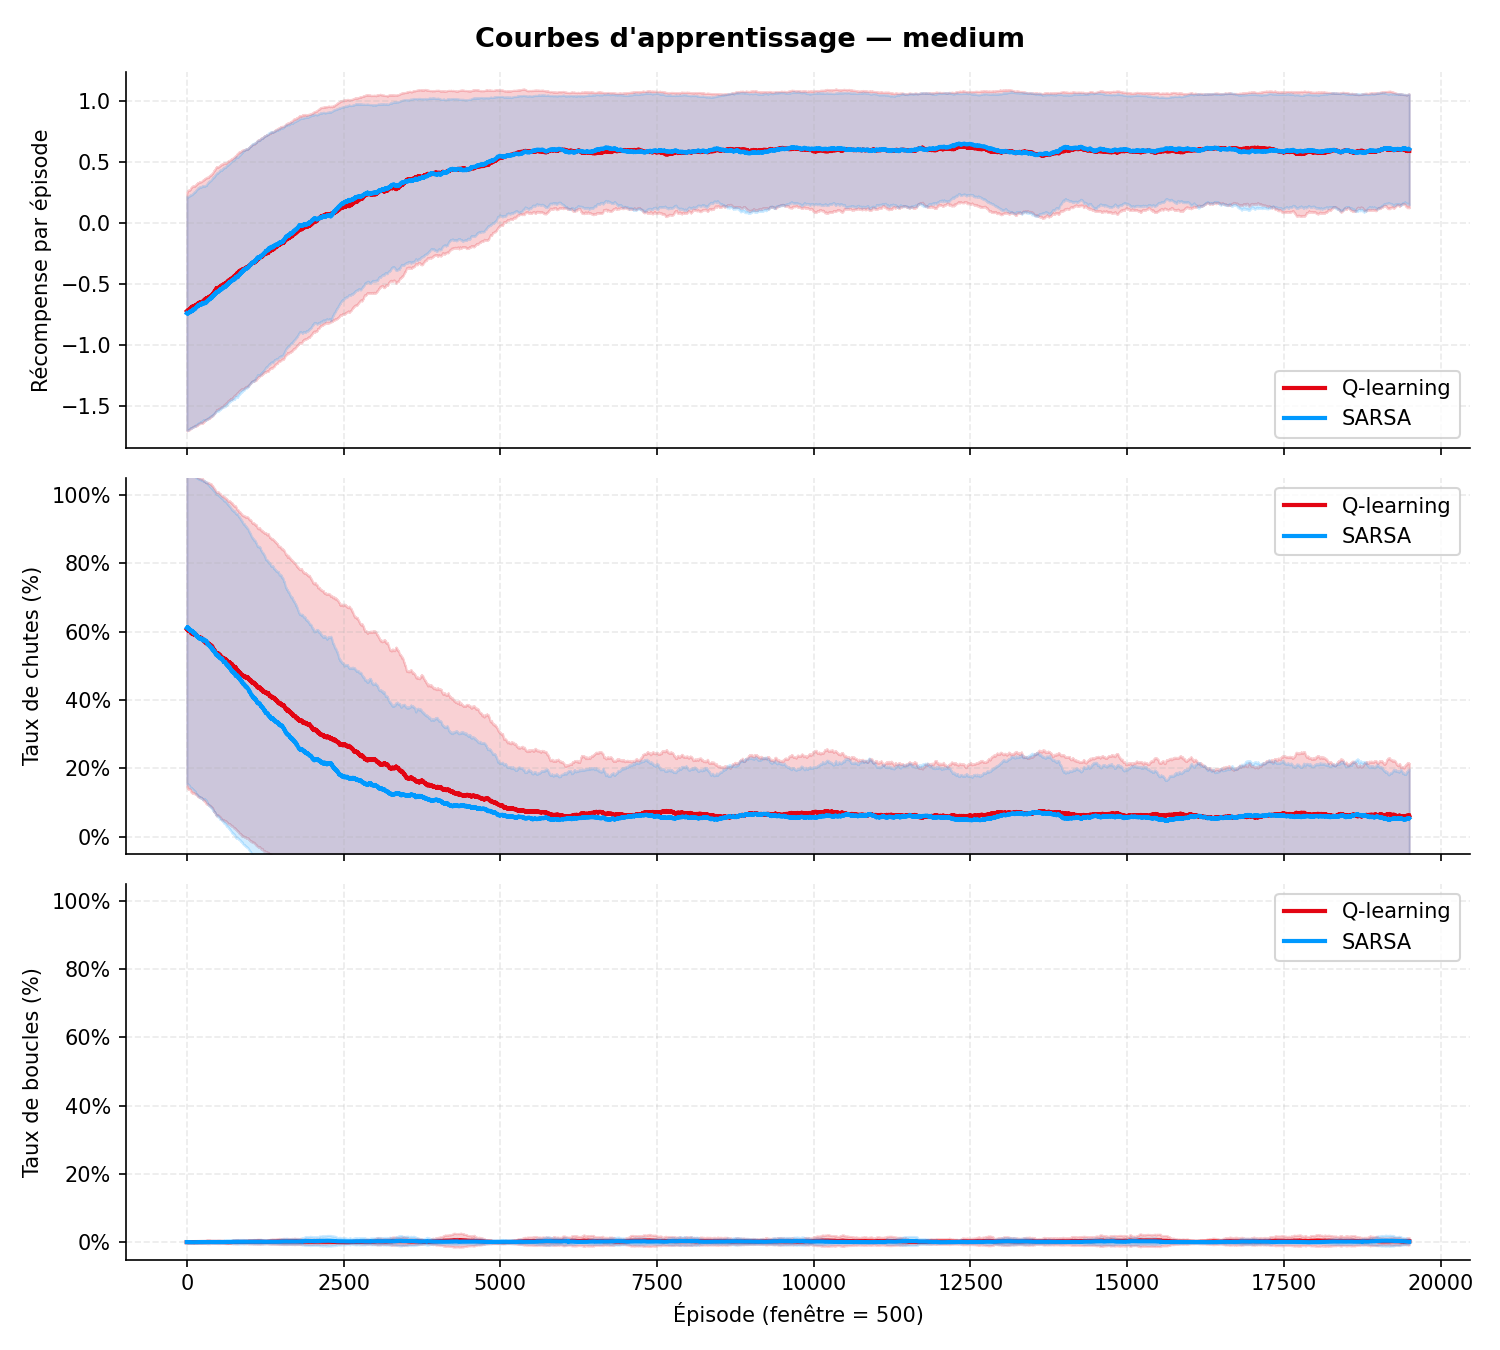
\includegraphics[width=\linewidth]{../figures/training_medium.png}
    \caption{\textbf{Moyen} --- La stochasticité fait bondir le taux de chutes initial. Le taux ne converge pas vers zéro : $\varepsilon_{\min}=5\%$ combiné aux glissades maintient un risque irréductible lié au bruit de transition.}
    \label{fig:train_medium}
  \end{subfigure}
  \caption{Courbes d'apprentissage (3 panneaux : récompense, chutes, boucles). Bande colorée~: $\pm$ un écart-type sur 10 répétitions.}
  \label{fig:train_easy_medium}
\end{figure}
\begin{figure}[H]
  \centering
  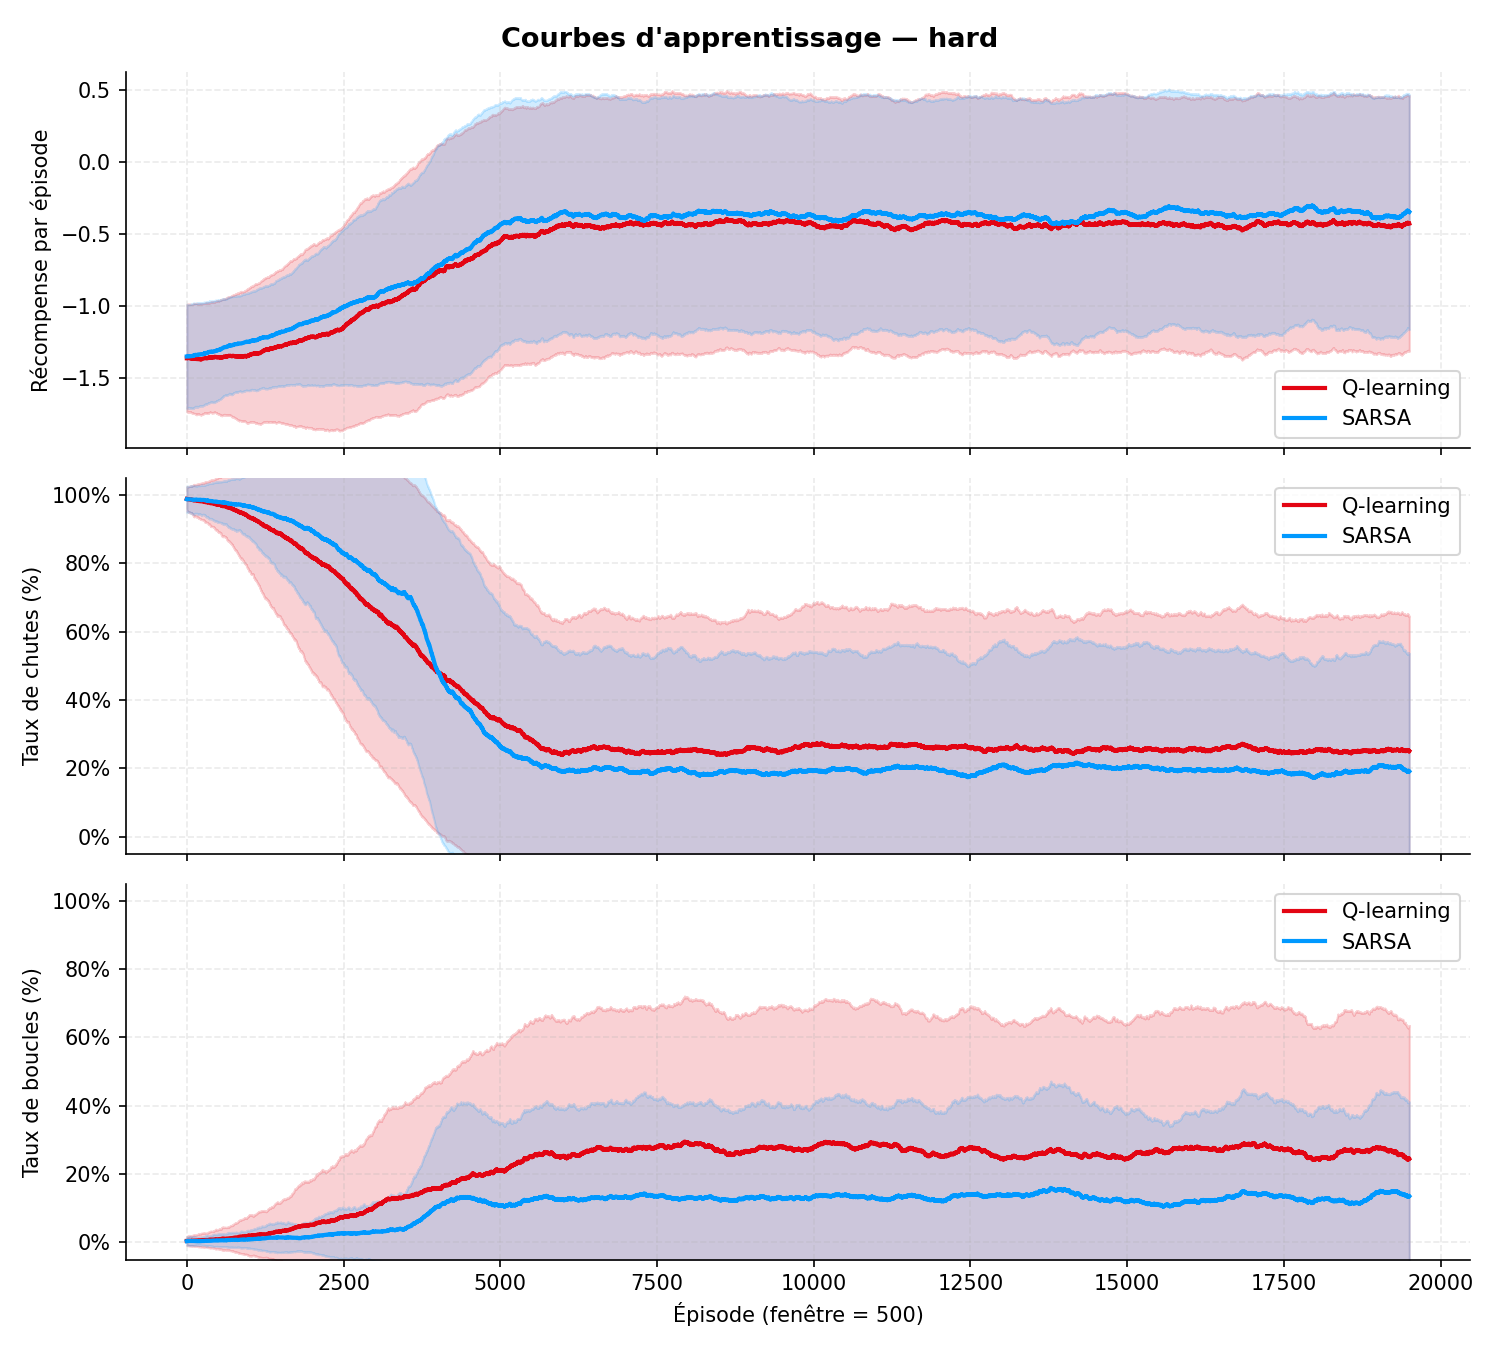
\includegraphics[width=0.48\linewidth]{../figures/training_hard.png}
  \caption{\textbf{Difficile} --- Les deux stratégies démarrent à un taux de chutes élevé, puis divergent : SARSA converge vers un taux de chutes et de boucles plus faible que Q-learning, reproduisant le phénomène de \textit{cliff walking}~\citep{sutton2018}. La mise à jour \textit{on-policy} intègre le coût de l'exploration et oriente l'agent vers le détour sûr.}
  \label{fig:train_hard}
\end{figure}
\begin{figure}[H]
  \centering
  \begin{subfigure}[t]{0.46\linewidth}
    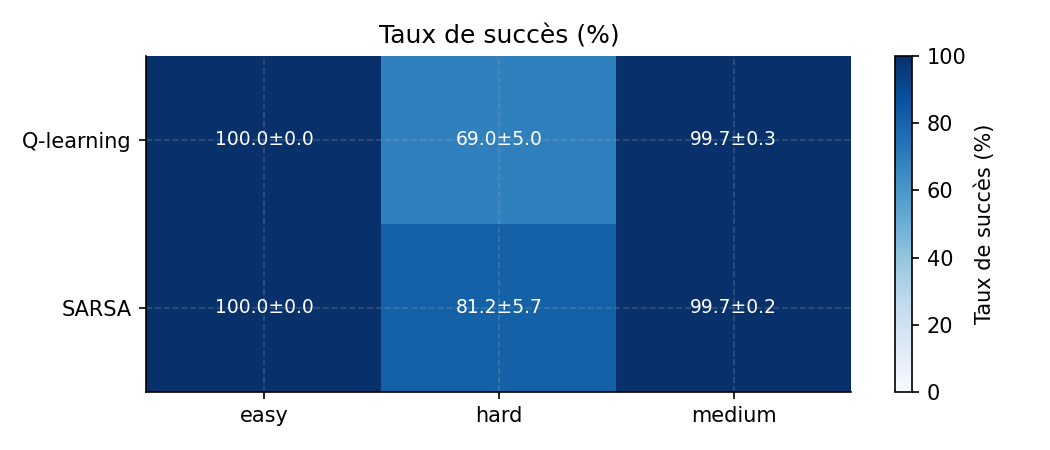
\includegraphics[width=\linewidth]{../figures/overview_success_rate.png}
    \caption{Taux de succès à l'évaluation (politique greedy, 500 épisodes). Les échecs sont exclusivement des boucles (dépassements de la limite de pas) — le taux de chutes est nul.}
    \label{fig:overview}
  \end{subfigure}
  \hfill
  \begin{subfigure}[t]{0.46\linewidth}
    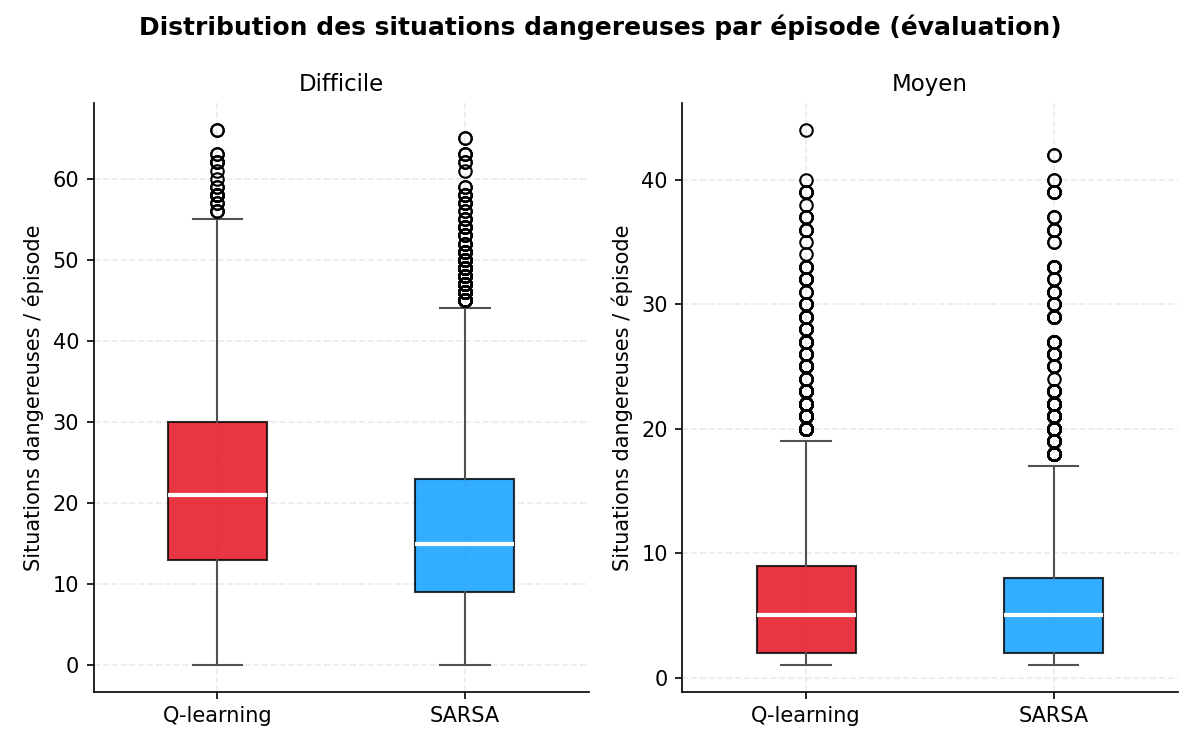
\includegraphics[width=\linewidth]{../figures/danger_boxplot.png}
    \caption{Distribution des situations dangereuses par épisode. Sur le cas Difficile, SARSA affiche une médiane plus basse et une variance moindre.}
    \label{fig:boxplot}
  \end{subfigure}
  \caption{Évaluation finale --- comparaison Q-learning vs SARSA.}
  \label{fig:eval_overview}
\end{figure}

Le Tableau~\ref{tab:eval} synthétise les indicateurs d'évaluation. Sur le cas Difficile, la divergence est marquée : Q-learning accumule $31{,}0\% \pm 5{,}0\%$ de boucles contre $18{,}8\% \pm 5{,}7\%$ pour SARSA ($+12{,}2$\,pts). SARSA réduit également la proximité aux trous ($25{,}9\%$ contre $29{,}9\%$) et emprunte nettement plus souvent le chemin sûr identifié par Dijkstra~\citep{dijkstra1959} ($70{,}4\% \pm 2{,}9\%$ contre $60{,}1\% \pm 2{,}9\%$, écart de $+10{,}3$\,pts), avec une variance identique confirmant la robustesse de cet avantage.

\begin{table}[H]
  \centering
  \caption{Indicateurs d'évaluation finale (politique greedy, 500 épisodes, moyenne $\pm$ écart-type, 10 répétitions). Chemin sûr : chevauchement $\geq 50\%$ avec le chemin Dijkstra (cas Difficile uniquement).}
  \label{tab:eval}
  \small
  \begin{tabular}{llccc}
    \toprule
    & & \textbf{Facile} & \textbf{Moyen} & \textbf{Difficile} \\
    \midrule
    \multirow{4}{*}{Q-learning}
      & Succès      & $100{,}0 \pm 0{,}0\%$ & $99{,}7 \pm 0{,}3\%$ & $69{,}0 \pm 5{,}0\%$ \\
      & Boucles     & $0{,}0 \pm 0{,}0\%$   & $0{,}3 \pm 0{,}3\%$  & $31{,}0 \pm 5{,}0\%$ \\
      & Danger      & $20{,}0 \pm 0{,}0\%$  & $28{,}5 \pm 1{,}6\%$ & $29{,}9 \pm 2{,}4\%$ \\
      & Chemin sûr  & ---                   & ---                  & $60{,}1 \pm 2{,}9\%$ \\
    \midrule
    \multirow{4}{*}{SARSA}
      & Succès      & $100{,}0 \pm 0{,}0\%$ & $99{,}7 \pm 0{,}2\%$ & $81{,}2 \pm 5{,}7\%$ \\
      & Boucles     & $0{,}0 \pm 0{,}0\%$   & $0{,}3 \pm 0{,}2\%$  & $18{,}8 \pm 5{,}7\%$ \\
      & Danger      & $20{,}0 \pm 0{,}0\%$  & $27{,}7 \pm 0{,}6\%$ & $25{,}9 \pm 2{,}2\%$ \\
      & Chemin sûr  & ---                   & ---                  & $70{,}4 \pm 2{,}9\%$ \\
    \bottomrule
  \end{tabular}
\end{table}

La Figure~\ref{fig:policy_hard} visualise directement les politiques greedy apprises sur le cas Difficile. Les flèches révèlent que SARSA dirige systématiquement l'agent vers les colonnes droites (contour Dijkstra en vert) avant de descendre vers G, tandis que Q-learning présente des flèches contradictoires dans la zone centrale — symptôme de boucles dues à une sous-estimation du risque de glissade. Ce résultat illustre concrètement la distinction \textit{off-policy}/\textit{on-policy} : Q-learning, optimiste, accumule des trajectoires circulaires ($31\%$ de boucles) ; SARSA, conservateur, apprend un détour cohérent ($18{,}8\%$).

\begin{figure}[H]
  \centering
  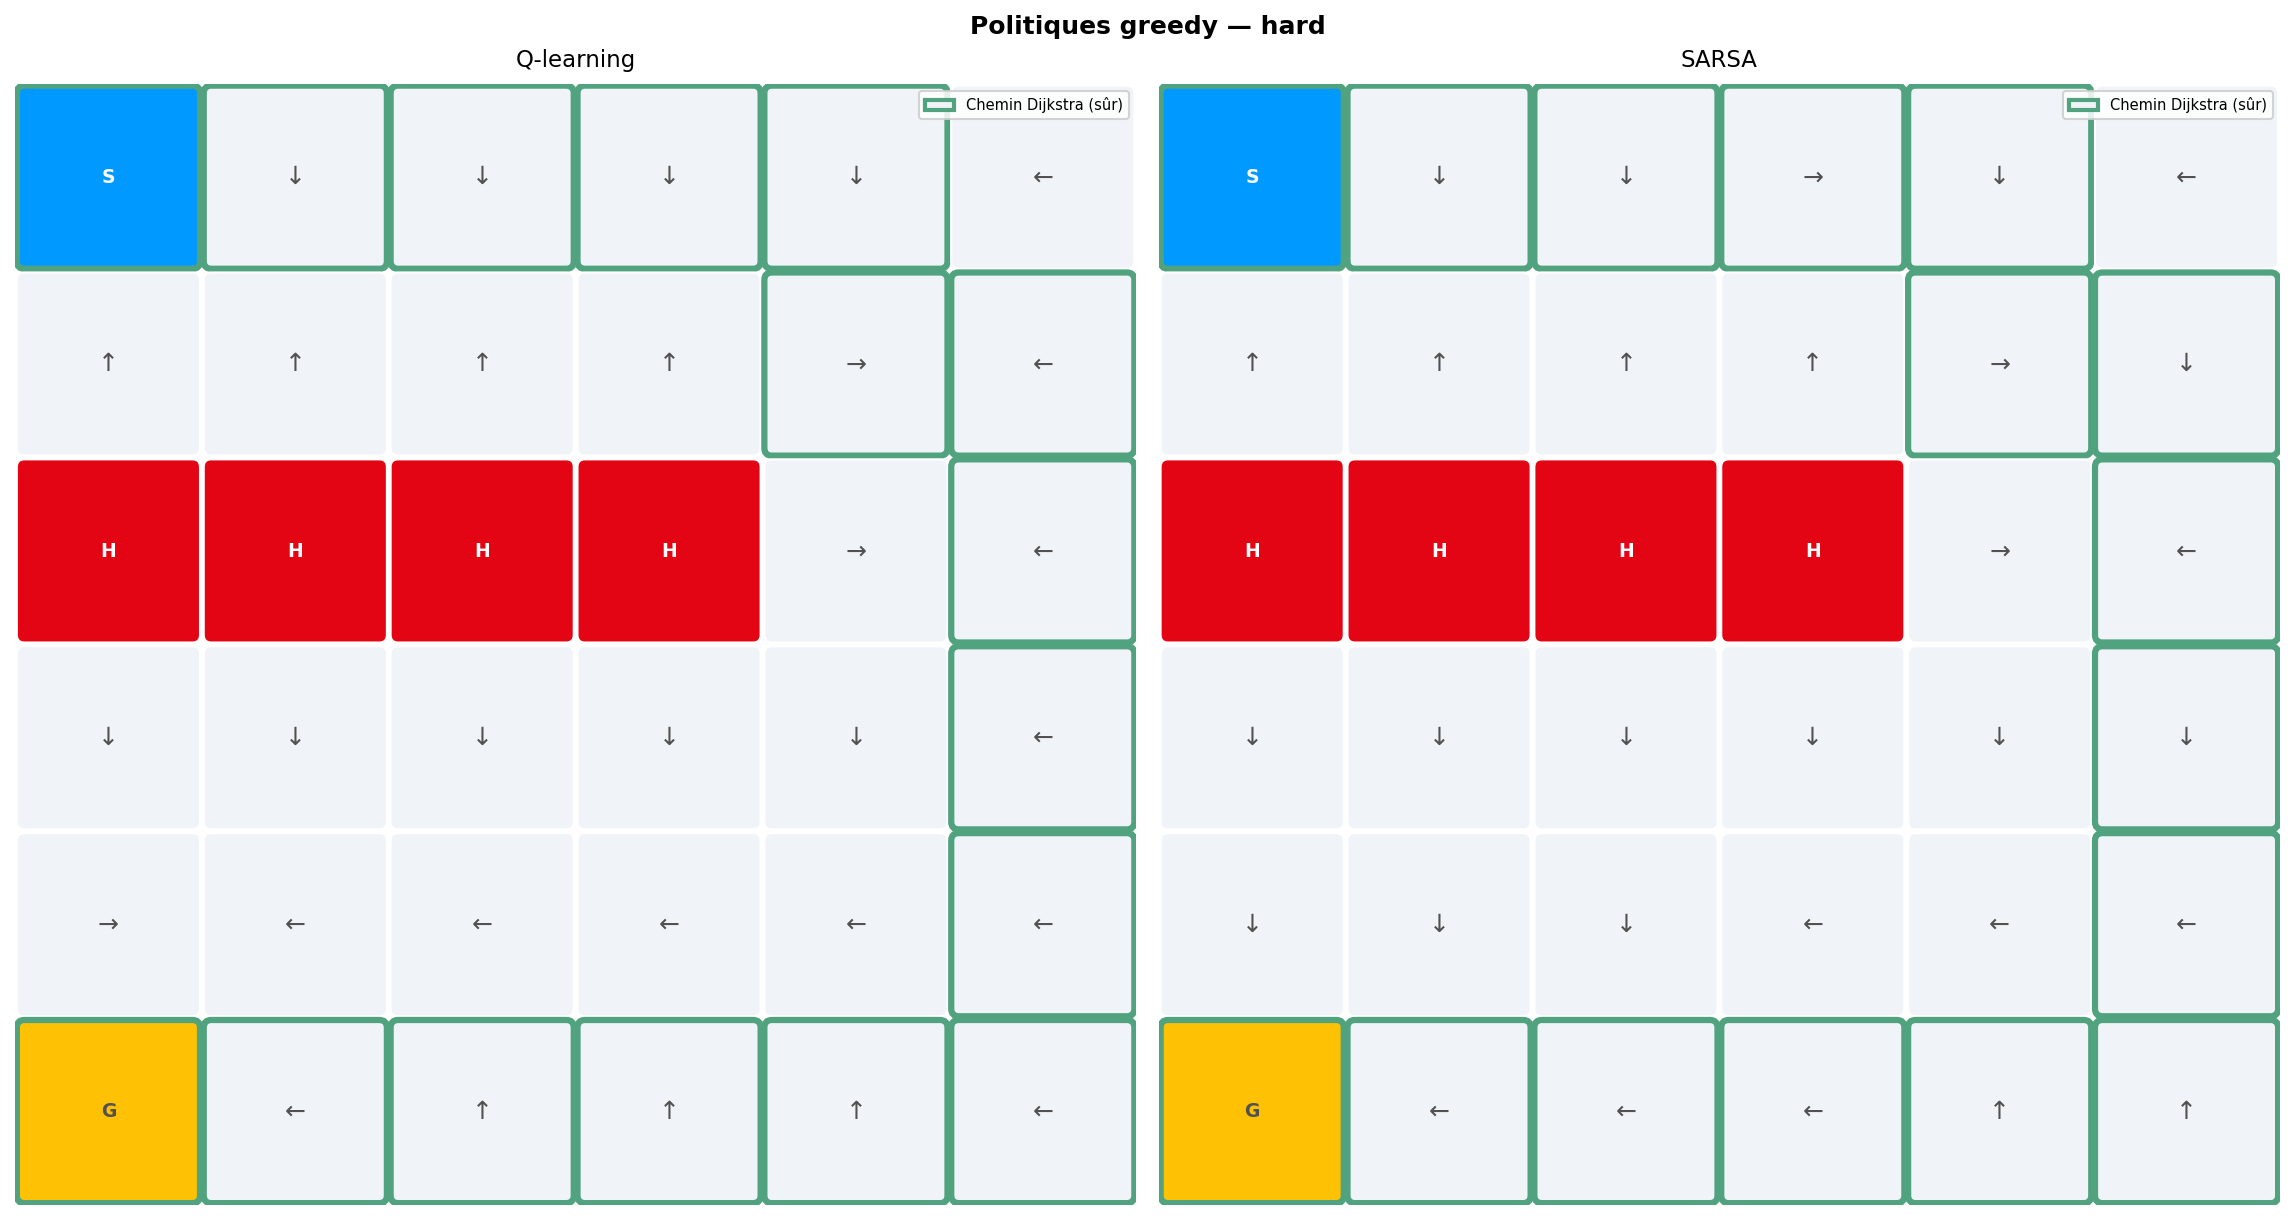
\includegraphics[width=\linewidth]{../figures/policy_hard.png}
  \caption{Politiques greedy apprises sur le cas Difficile (moyenne sur 10 répétitions). Les flèches indiquent l'action greedy dans chaque état libre ; le contour vert délimite le chemin de référence Dijkstra. SARSA emprunte le détour sûr plus systématiquement que Q-learning.}
  \label{fig:policy_hard}
\end{figure}

En somme, Q-learning converge légèrement plus vite en début d'apprentissage mais au prix d'une instabilité persistante : plus de boucles ($31\%$ contre $18{,}8\%$), une plus grande proximité aux trous ($29{,}9\%$ contre $25{,}9\%$) et une politique qui emprunte moins souvent le détour sûr ($60{,}1\%$ contre $70{,}4\%$). SARSA, plus conservateur grâce à sa mise à jour \textit{on-policy}, apprend un comportement plus sûr et plus cohérent. Ces observations soulignent les limites fondamentales des méthodes TD sans mécanisme explicite d'évitement du danger, et motivent l'introduction d'une telle approche dans le rapport final.

\newpage
\bibliographystyle{unsrtnat}
\bibliography{references}

\end{document}
